\documentclass{article}
\usepackage[paperwidth=6in,paperheight=3.9in,margin=0in]{geometry}
\usepackage{mathptmx}%{times}
\usepackage{graphicx}
\usepackage{siunitx}
\usepackage[absolute,overlay]{textpos}
\usepackage{color}

\setlength{\parindent}{0pt}
\begin{document}
\TPMargin{1pt}
\begin{textblock}{4}(1.4,0.8)
\normalsize
(a) BTF linearUpwind \\
\hspace*{1em}$\ell_2 = \num{1.234}$
\hspace*{1em}$\ell_\infty = \num{1.234}$
\end{textblock}
\begin{textblock}{4}(6.5,0.8)
\normalsize
(b) Cut cell linearUpwind \\
\hspace*{1em}$\ell_2 = \num{1.234}$
\hspace*{1em}$\ell_\infty = \num{1.234}$
\end{textblock}
\begin{textblock}{4}(11.5,0.8)
\normalsize
(c) Slanted cell linearUpwind \\
\hspace*{1em}$\ell_2 = \num{1.234}$
\hspace*{1em}$\ell_\infty = \num{1.234}$
\end{textblock}
\begin{textblock}{4}(1.4,7.3)
\normalsize
(d) BTF cubicFit \\
\hspace*{1em}$\ell_2 = \num{1.234}$
\hspace*{1em}$\ell_\infty = \num{1.234}$
\end{textblock}
\begin{textblock}{4}(6.5,7.3)
\normalsize
(e) Cut cell cubicFit \\
\hspace*{1em}$\ell_2 = \num{1.234}$
\hspace*{1em}$\ell_\infty = \num{1.234}$
\end{textblock}
\begin{textblock}{4}(11.5,7.3)
\normalsize
(f) Slanted cell cubicFit \\
\hspace*{1em}$\ell_2 = \num{1.234}$
\hspace*{1em}$\ell_\infty = \num{1.234}$
\end{textblock}
\includegraphics{../mountainAdvection-btf-6km-linearUpwind-1000/10000/errorContoursW.pdf}
\hspace*{0.35em}
\includegraphics{../mountainAdvection-cutCell-6km-linearUpwind-1000/10000/errorContours.pdf}
\hspace*{0.35em}
\includegraphics{../mountainAdvection-slantedCell-6km-linearUpwind-1000/10000/errorContours.pdf} \\
\includegraphics{../mountainAdvection-btf-6km-cubicUpwind-1000/10000/errorContoursSW.pdf}
\includegraphics{../mountainAdvection-cutCell-6km-cubicUpwind-1000/10000/errorContoursS.pdf}
\includegraphics{../mountainAdvection-slantedCell-6km-cubicUpwind-1000/10000/errorContoursS.pdf} \\
\centering
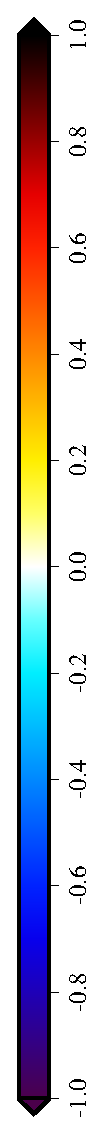
\includegraphics[height=5.5in,angle=270]{mountainAdvectionErrorLegend.eps}
\end{document}
